\chapter{Manutenção e seus Conceitos}
\label{cap-manutencao}

A manutenção pode ser considerada a atividade que mais passou por mudanças nos últimos anos. Isso é resultado da complexidade e diversidade das tarefas que devem ser realizadas pelos seus responsáveis. O aumento na diversidade de equipamentos eletrônicos que dão suporte a atividades corriqueiras e essenciais, e devem ser mantidos, é um dos grandes desafios que deve ser encarado pelas empresas e organizações.

Equipamentos eletrônicos estão presentes em todos os momentos do cotidiano de uma empresa, seja um computador, uma televisão, um projetor, entre outros. Como mantê-los de forma que eles sejam nossos aliados e não nossos inimigos? A resposta está em evoluir a manutenção junto com a quantidade e diversidade dos ativos da sua empresa.
	
Um trecho da introdução do livro de Kardec e Nascif, Manutenção - Função Estratégica, chama atenção por descrever exatamente a mudança primordial exigida no setor de manutenção, se o para paradigma anterior, e ainda atual na maioria das empresas, era: \lq\lq O homem de manutenção sente-se bem quando executa um bom reparo \rq\rq, o novo paradigma é: \lq\lq O homem de manutenção sente-se bem quando não tem que fazer reparo porque conseguiu evitar todas as quebras não planejadas \rq\rq.
	
A manutenção irá extrapolar o seu próprio significado, que de acordo com o BSI \cite{british1993bs} é \lq\lq A combinação de todas as ações técnicas e administrativas associadas destinadas a reter um item ou restaurá-lo em um estado no qual possa desempenhar sua função requerida \rq\rq. Manutenção será atrelada a inovação e não apenas a preservação do estado de um ativo. É preciso pensar em como evitar e prever, o mau funcionamento, parada ou até perda de um ativo.
	
Como então alinhar a manutenção aos objetivos da organização, fazendo dela uma ferramenta poderosa de preservação e aumento do tempo de vida dos ativos da organização, resultando na diminuição de custos com consertos on demand, atividades paradas, entre outros. Este capítulo apresentará tipos de manutenções disponíveis, sobre gerenciamento de manutenção e suas aplicações.

%------------------------------------------------------------------------------------------------%

\section{Tipos de Manutenção}
\label{tipos-man}


Kardec e Nascif citam seis tipos de manutenção, que de forma geral englobam os tantos outros existentes. A Figura~\ref{tiposmanutencao}, mostra como os tipos de manutenção se relacionam, segundo os autores. 
Também serão mostrados os objetivos e vantagens de se aplicar essas estratégias de manutenção, segundo \cite{pereira2011engenharia}.

\graphicspath{{figuras/}}
\begin{figure}[H]
\centering
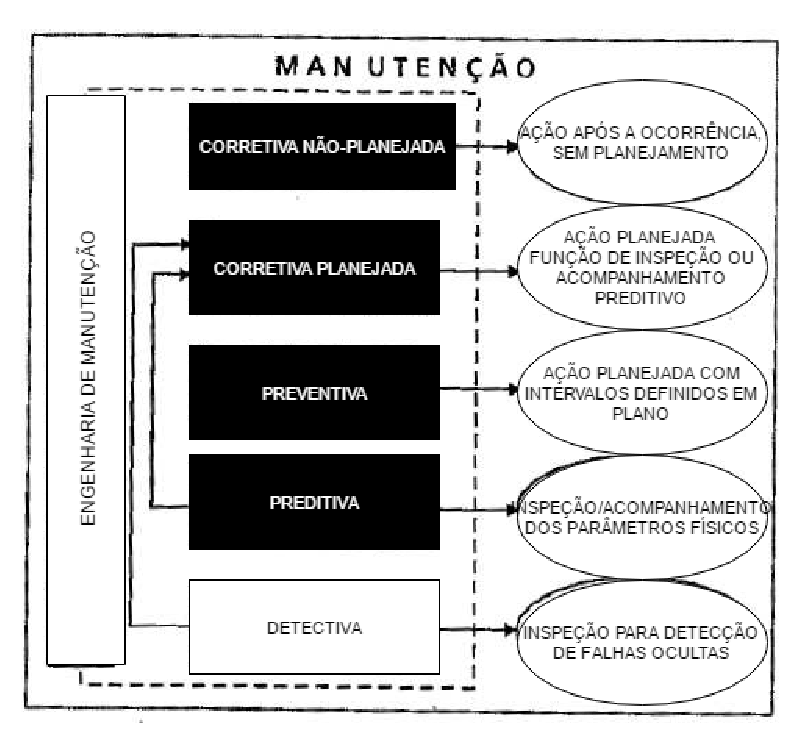
\includegraphics[width=0.8\textwidth]{tipos-de-manutencao}
\caption{Tipos de Manutenção. \textbf{Fonte: Manutenção - Função Estratégica, 2009, pg. 38\hfill}}
\label{tiposmanutencao}
\end{figure}

%--------------------------------------------%

\subsection{Manutenção Corretiva}

		\emph{"Manutenção Corretiva é a atuação para a correção da falha ou do desempenho menor do que esperado."} \cite{kardecnascif2010}

		\emph{"Manutenção realizada após uma falha destinada a colocar um item em um estado onde possa executar uma função necessária de forma segura e eficiente"} \cite{british1993bs}

		Ocorre em equipamentos com defeito ou que estão funcionando de forma diferente do esperado. Sua principal ação é Corrigir ou Restaurar para o estado de funcionamento. Pode ser Planejada ou Não Planejada.

		\begin{itemize}
			\item \textbf{Manutenção Corretiva Não Planejada:} configura na correção da falha realizada de forma aleatória, após a o fato já ocorrido. Acarreta em custos altos, com a própria ação da correção, perda de qualidade do equipamento, interrupção das atividades onde o equipamento é necessário.
			\item \textbf{Manutenção Corretiva Planejada:} configura na correção da falha realizada de forma aleatória, após a o fato já ocorrido. Acarreta em custos altos, com a própria ação da correção, perda de qualidade do equipamento, interrupção das atividades onde o equipamento é necessário.
		\end{itemize}

		\textbf{Objetivos da Manutenção Corretiva}
			\begin{itemize}
				\item Reparar de imediato a ocorrência da falha ou defeito de um equipamento;   
				\item Reduzir  o tempo de  parada de um processo produtivo ou equipamento que apresente falha ou defeito; 
				\item Impedir o aumento dos danos; 
				\item Aproveitar a vida útil estimada dos componentes e de um equipamento.
			\end{itemize}	

		\textbf{Vantagens}

		A manutenção corretiva apresenta uma vantagem importante: é uma boa solução para processos produtivos não contínuos e que o tempo de parada para reparo é curto. 

%--------------------------------------------%

\subsection{Manutenção Preventiva}

		\emph{"Manutenção Preventiva é a atuação realizada de forma a reduzir ou evitar a falha ou queda no desempenho, obedecendo a um plano previamente elaborado, baseado em intervalos definidos de tempo."} \cite{kardecnascif2010}

		A manutenção preventiva busca evitar a ocorrência de falhas. Sua adoção é mais adequada quando a reposição de equipamentos for simples, tiver custo alto de falhas e as falhas forem mais prejudiciais as atividades.


		\textbf{Objetivos da Manutenção Preventiva}
			\begin{itemize}
				\item Prever, antecipadamente, quando provavelmente ocorrerá a falha ou defeito em um equipamento;    
				\item Aumentar o tempo de disponibilidade dos equipamentos; 
				\item Aproveitar a vida útil estimada dos componentes e de um equipamento; 
				\item Aumentar o grau de confiança no desempenho de um equipamento. 
			\end{itemize}

		\textbf{Vantagens}
			\begin{itemize}
				\item Antecipar o reparo através da manutenção corretiva antes da falha ou do defeito;    
				\item Aumentar o tempo de disponibilidade dos equipamentos; 
				\item Reduzir o trabalho de emergência não planejado; 
				\item Impedir o aumento dos danos; 
				\item Aumentar o grau de confiança no desempenho de um equipamento.
			\end{itemize}

%--------------------------------------------%

\subsection{Manutenção Preditiva}

		\emph{"Manutenção Preditiva é a atuação realizada com base em modificações de parâmetros de condição ou desempenho, cujo acompanhamento obedece a uma sistemática."} \cite{kardecnascif2010}

		Visa a operação contínua do equipamento por mais tempo possível, as medições e verificações são realizadas com o equipamento em produção, ou seja, com ele funcionando e operando na suas atividades. 

		Segundo Kardec e Nascif, indica-se na adoção da manutenção preditiva a análise dos fatores abaixo:

			\begin{itemize}
				\item Aspectos relacionados com a segurança pessoal e operacional.
				\item Redução de custos pelo acompanhamento constante das condições dos equipamentos, evitando assim intervenções desnecessárias.
				\item Manter os equipamentos operando, de modo seguro, por mais tempo.
			\end{itemize}

		\textbf{Objetivos da Manutenção Preditiva}

			\begin{itemize}
				\item Determinar, antecipadamente, a necessidade de serviços de manutenção em uma peça específica de um equipamento;  
				\item Aumentar o tempo de disponibilidade dos equipamentos;
				\item Reduzir o trabalho de emergência não planejado;  
				\item Aproveitar a vida útil total dos componentes e de um equipamento.
			\end{itemize}

		\textbf{Vantagens}

			\begin{itemize}
				\item Aumento da vida útil do equipamento; 
				\item Controle dos materiais (peças, componentes, partes, etc.) e melhor gerenciamento; 
				\item Diminuição dos custos nos reparos.
			\end{itemize}
		
%--------------------------------------------%

\subsection{Manutenção Detectiva ou Proativa}

		\emph{"Manutenção Detectiva é a atuação efetuada em sistemas de proteção buscando detectar falhas ocultas ou não perceptíveis ao pessoal de operação e manutenção."} \cite{kardecnascif2010}

		Detectar falhas ocultas é fundamental para garantir a confiabilidade, os especialistas verificam o sistema sem tirá-lo de operação, detectam falhas ocultas e podem corrigir a situação, com o sistema operando.

		Tem como base a frequência na ocorrência da falha. É feito um histórico dessas ocorrências no equipamento e retiradas informações para saber qual a causa básica de falhas frequentes. Ela gera ações que estão relacionadas a causa raiz da falha, com o objetivo de aumentar o tempo de vida do equipamento.

		\textbf{Objetivos da Manutenção Detectiva}

			\begin{itemize}
				\item Localização dos possíveis indícios ocultos que podem levar a uma avaria; 
				\item Aproveitar a vida útil total dos componentes e de um equipamento.
			\end{itemize}

		\textbf{Vantagens}	

			\begin{itemize}
				\item Limitação da quantidade de peças de reposição; 
				\item Controle dos materiais (peças, componentes, partes, etc.) e melhor gerenciamento.
			\end{itemize}

%--------------------------------------------%

\section{Engenharia de Manutenção}

Mencionados os principais tipos de manutenções descritos na literatura, cabe a engenharia de manutenção definir um planejamento das tarefas e técnicas que devem ser aplicadas, pois não há um tipo de manutenção que é adequado a todo o universo de máquinas, equipamentos ou peças que se desejam conservar. Cabendo ao contexto do uso em que esses ativos são utilizados, e outros fatores, a definição da melhor técnica de manutenção a ser empregada.

Em síntese a atuação da engenharia de manutenção é vocacionada na aplicação dos conceitos de otimização dos equipamentos, dos processos e dos orçamentos, de modo a alcançar uma melhor manutenibilidade, fiabilidade e disponibilidade dos equipamentos. 

A análise das ferramentas de gestão e das técnicas de otimização da manutenção aumentam a disponibilidade dos equipamentos e instalações, na medida em que aplicam os conhecimentos da engenharia de manutenção \cite{xenos1998gerenciando}. Dentre as teorias comumente defendidas, temos a da \lq\lq curva da banheira \rq\rq, que confronta em um gráfico bidimensional o tempo de uso versus a taxa de falhas dos equipamentos, conforme mostra a figura~\ref{Curva da banheira}.

\graphicspath{{figuras/}}
\begin{figure}[H]
\centering
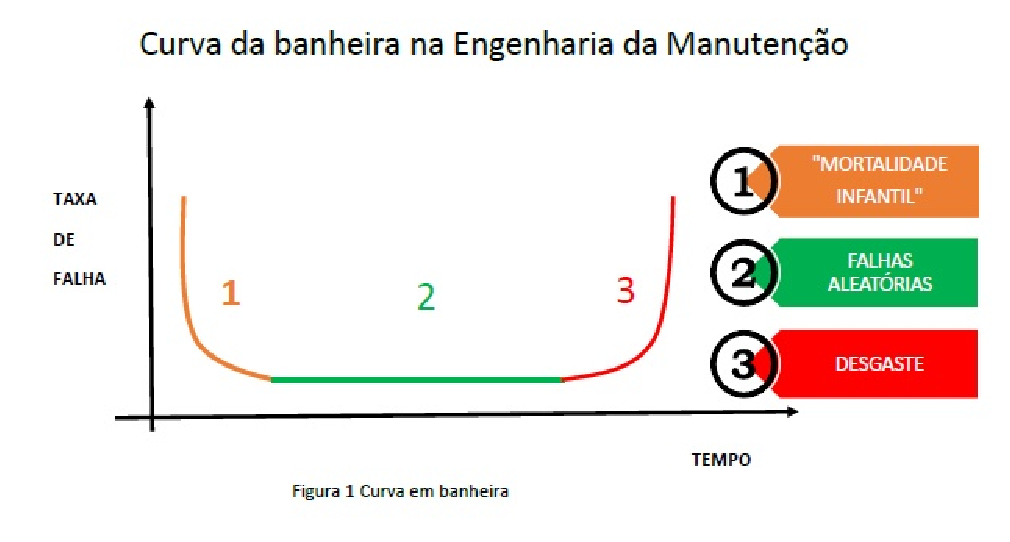
\includegraphics[width=0.8\textwidth]{curva_da_banheira.eps}
\caption{Teoria da curva da banheira \textbf{Fonte:A Curva da Banheira na Engenharia da Manutenção:2016.}}
\label{Curva da banheira}
\end{figure}

Conforme observado no gráfico acima, as frequências de ocorrência das falhas em um equipamento podem ser classificadas em 1) decrescente; 2) constante ou aleatória e 3) crescente, estando associadas ao estágio do ciclo de vida do equipamento.

\begin{itemize}
	\item \textbf{1) Decrescente:} Nesta fase, também denominada de \lq\lq mortalidade infantil \rq\rq, ocorrem falhas advindas dos defeitos de projeto, de fabricação e de instalação. É caracterizada por uma alta taxa de falha no início de sua operação;
	\item \textbf{2) Constante ou aleatória:} Esta fase costuma ser denominada de vida normal ou fase de estabilidade do equipamento, uma vez que a taxa de falhas é aproximadamente constante e ocorrem aleatoriamente, estando associadas a aplicação de esforços acidentais e/ou erros de manutenção. A taxa de falha é menor do que nas demais fases;
	\item \textbf{3) Crescente:} Esta fase reflete o período de instabilidade próprio do fim da vida útil do equipamento, ou seja, o sistema e seus componentes apresentam falhas por desgaste natural, decorrente do seu uso. Há um aumento considerável da taxa de falha nesta fase.  
\end{itemize} 

O conhecimento da \lq\lq curva da banheira \rq\rq por parte das instituições auxilia no controle da manutenção, na determinação da vida útil, no estabelecimento do tempo de garantia e na adoção de medidas indispensáveis para o aumento da disponibilidade e confiabilidade dos equipamentos.

Bem assim, os gestores de manutenção baseados nos conhecimentos já expostos devem primeiramente buscar a definição de qual tipo de manutenção será usada em cada modelo de equipamento, e para tal devem fazer uso de algoritmos. A Figura~\ref{melhor_tecnica_de_manutencao} mostra um dos possíveis fluxogramas para definição do tipo de manutenção.

Na sequência de instruções demonstrada pela figura~\ref{melhor_tecnica_de_manutencao}, são levados em conta em grau de importância a segurança do trabalhador, do meio ambiente e do patrimônio, além das questões operacionais, ou seja, o quanto uma falha no equipamento impacta em custo, qualidade e tempo de reparo.

A ideia central é que, a partir do momento em que ocorra a avaria, todas as questões citadas sejam analisadas de forma lógica, para depois fazer uso de uma das três abordagens de manutenção: manutenção corretiva, preditiva ou preventiva.

\begin{landscape}
\graphicspath{{figuras/}}
\begin{figure}[H]
\centering
\includegraphics[width=1.5\textwidth]{melhor_tipo_manutencao.eps}
\caption{Sistemática para avaliação da melhor técnica de manutenção. \textbf{Fonte: \cite{neumann2013gestao} adaptada pelo autor}}
\label{melhor_tecnica_de_manutencao}
\end{figure}
\end{landscape}

\subsection{Modelagem da falha de equipamentos}

Embora a maioria das causas que levam os equipamentos ao desgaste estejam ligadas a seu uso, eventualmente, podem ter ocorrido problemas durante o seu processo de fabricação, ocasionando a produção de componentes fora da especificação e mais frágeis. Estes equipamentos quais provavelmente irão apresentar problemas prematuros, quando colocados em operação. De acordo com Sanches (2010, p. 19) os equipamentos que apresentam defeitos/falhas provenientes dos processos de fabricação apresentam problemas em um período inicial, que em média corresponde à 5\% da sua vida útil – período conhecido como falhas prematuras ou precoces.

Ou quando se deseja melhorar as suas condições de uso, algumas delas estão relacionadas à escolha do equipamento mais indicado, ou quais modificações serão necessárias a serem feitas na infraestrutura para adequadamente utilizá-lo.

Restabelecer características construtivas originais dos equipamentos, garantindo a eles um nível de desempenho esperado através da manutenção. 
Estas ações de correição e prevenção quando adotadas aumentam a eficiência operacional e o tempo de vida útil dos ativos da organização. 

Koren e Krishna \cite{koren2007} dizem em seu livro \emph{Fault-Tolerant System} que todo tipo de tolerância a falhas é um exercício de explorar e gerenciar redundância. Redundância é a propriedade de ter mais de um recurso do que o minimamente necessário para o trabalho sendo feito. Quando acontece uma falha, a redundância é explorada par mascarar ou contornar essas falhas, mantendo o nível desejado de funcionalidade. Eles trazem quatro tipos de redundância: de hardware, de software, de informação e de tempo. Abaixo será relatado como os autores tratam os conceitos relacionados a \textbf{tolerância a falhas}. 

A tolerância a falhas tem como objetivo tornar máquinas mais confiáveis, por isso ela tem medidas próprias. Medida é uma abstração matemática, que expressa uma observação da performance de um objeto. O truque em definir medidas adequadas é manter o subsistema largo o suficiente para que o comportamento de interesse do usuário seja capturado, e ainda assim não tão largo, para que a medida não perca o foco.

%------------------------------------------------------------------------------------------------------------------------%

\section{Manutenção no Brasil}

Com o reconhecimento da importância de se empregar processos efetivos de manutenção nas organizações, surgiu nos anos setenta, Associações de Manutenção, na Espanha, México e Portugal, que despertou o interesse em profissionais brasileiros pelos conceitos, métodos e tecnologias que essa área dispõe. Em 1938, no III Congresso Ibero-Americano de Manutenção, foi aprovada a proposta de uma entidade no Brasil. Foi fundada então, em 17 de outubro de 1984, a \textbf{Associação Brasileira de Manutenção}, mudando seu nome em 2012 para \textbf{Associação Brasileira de Manutenção e Gestão de Ativos}. No começo, a ABRAMAN só tinha representantes dos setores de petróleo, eletricidade, siderurgia e transportes. Mais tarde a associação ganhou aderência por parte de setores diversos, por exemplo, hoje em dia a ABRAMAN emite certificados MBA de gestão de ativos para Instituições de Ensino Superior, assim como para outros setores. 

Em 1983, o IBP (Instituto Brasileiro de Petróleo) criou um documento nacional para análise da situação da manutenção no Brasil, a responsabilidade da elaboração passou para ABRAMAN desde a criação da associação em 1984, que em 1993, aderiu aos moldes de apresentação e desenvolvimento da AEM (Associação Espanhola de Manutenção), o qual é mantido até os dias de hoje.  

O Documento Nacional - A Situação da Manutenção no Brasil, apresenta resultados de pesquisas realizadas bienalmente, desde 1985, com indicadores de performance da Manutenção e Gestão de Ativos, presentes nos principais setores de produtos e serviços que movimentam a economia brasileira. No site da ABRAMAN \cite{abraman}, onde constam essas informações, também relata que um dos insumos para o documento são pesquisas e levantamento de índices em áreas de enfoque como \emph{Forma de Atuação, Nível Hierárquico, Pessoal Próprio, Quadro Técnico, Rotatividade e Contratação de Pessoal, Contratação e Conceito dos Serviços, Critérios na Contratação, Composição dos Custos, Aplicação dos Recursos - Pessoal, Qualidade na Manutenção, Custo por Faturamento, Disponibilidade Operacional, Idade Média, Valor de Estoque e Segurança Industrial}. O documento tem uma alta relevância por representar de forma detalhada uma análise da situação da função no Brasil. Tendo servido como fonte de dados para profissionais, estudantes, pesquisadores e gerentes de empresas.

Em uma de suas últimas pesquisas, no ano de 2013, a ABRAMAN revelou que o custo total da manutenção representou em média 4,69 por cento do faturamento bruto nas empresas brasileiras, perfazendo uma parcela significativa do PIB nacional, na verdade o valor mais alto dessa estatística desde o inicio da série histórica, iniciada em 1995, conforme mostra a Figura~\ref{custo_anual_2013}.

\graphicspath{{figuras/}}
\begin{figure}[H]
\centering
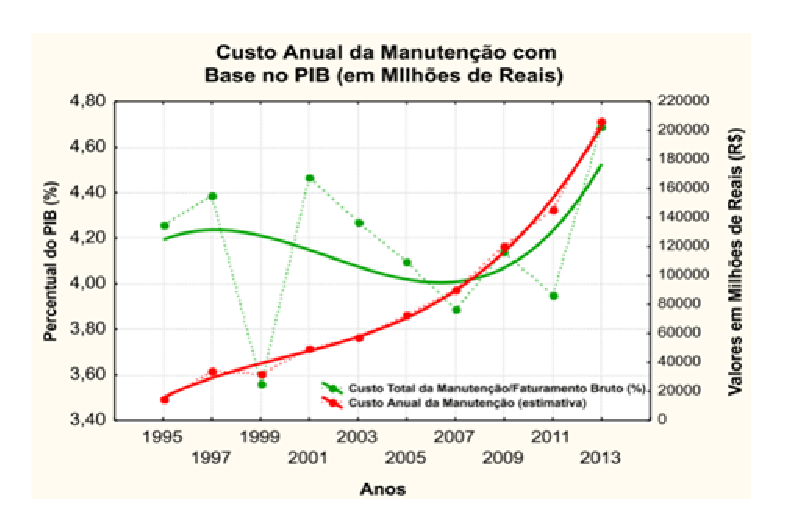
\includegraphics[width=0.8\textwidth]{dados_pib_pesquisa_intro.eps}
\caption{Custo anual da manutenção com base no PIB. \textbf{Fonte: ABRAMAN, Documento Nacional 2013.}}
\label{custo_anual_2013}
\end{figure}

Isto está aliado ao que afirma DEKKER \cite{dekker1998}, que relata que os gastos com manutenção tendem a crescer em todos os setores da economia, a despeito do desenvolvimento tecnológico, o que provocaria pensar que é uma contradição, porém as principais causas são a contínua expansão dos bens de capital e as exigências de mercado que impõe uma alta taxa de disponibilidade e confiabilidade dos equipamentos.

Dado essas informações, considerar a manutenção somente uma atividade operacional, é não enxergar o valor significativo envolvido nessa área, nem sua responsabilidade para com a qualidade e imagem da organização. A função da manutenção deve possuir políticas e estratégias para que ela tenha a mesma relevância que outras funções da organização, atribuindo-lhe diretrizes e metas.	

No setor público, às políticas de gestão da manutenção, como a de muitas outras áreas, tendem a evoluir em menor velocidade que na iniciativa privada, devido suas características legais e burocráticas que, apesar de necessárias para combater as práticas patrimonialistas, acabam por dificultar a inovação gerencial. Contudo o Estado precisa de um modelo de administração que traga resultados efetivos gastando a menor quantidade de recursos possíveis.

%--------------------------------------------------------------------------------------------------------%

\chapter{Ativos, Gestão de Ativos e Normas}
\label{cap-ativos}

Esse capítulo busca explanar sobre ativos, como geri-los e quais normas e padrões existem para fazê-lo. É importante entender o que é um ativo e qual a sua importância em uma empresa. Saber manipulá-los de forma correta pode ser uma forma valiosa de economia e maior rendimentos das atividades cotidianas, complexas e indispensáveis.

\section{Ativos}

\textbf{Definição:} \emph{Dentro da contabilidade, ativo é um recurso econômico. Pode ser considerado qualquer coisa tangível ou intangível. Expressa bens, valores créditos, direitos e assemelhados, que podem gerar valor econômico. Formam o patrimônio de uma pessoa singular ou coletiva e são avaliados pelo seu custo.} \cite{sullivan2003}\cite{fulgencio2007} 

\textbf{Definição:} \emph{Ativo físico é algo que tem valor real ou potencial para uma organização.
Exemplos: plantas, instalações, equipamentos, estoques, ferramentas, materiais, edifícios, veículos etc.} \cite{nicolay2015}

\textbf{Definição:} \emph{Ativo é um item, coisa ou entidade que tem potencial ou valor real para uma organização.} (iso 55000)

Ativos são recursos que dão suporte as atividades realizadas por uma organização. E pelas definições acima constata-se que são intrínsecos ao seu custo e também geram valor para o negócio. A troca constante desses ativos, por obsolescência, quebra ou falhas, podem gerar custos altos e despesas extras. Por isso é necessário geri-los de forma adequada, de forma a preservá-los, a prolongar seu tempo de vida e ter uma previsão dos gastos necessários para mantê-los. 

Controlar seu ciclo de vida pode ser uma forma de prever falhas, evitá-las e assim melhorar seu desempenho e aumentar seu tempo de uso. A gestão de ativos é uma área que vem sendo valorizada exatamente porque a indústria percebeu a necessidade de diminuir os custos com reparos e substituições.

Marcio Nicolay \cite{nicolay2015} defini vida do ativo e ciclo de vida como:

\textbf{Vida do ativo:} é o período compreendido desde sua criação até o final de sua vida. Sua vida não necessariamente termina depois do descarte.

\textbf{Ciclo de vida:} são todas as etapas envolvidas na gestão de um ativo. Quantidade de etapas e duração variam de acordo com a necessidade da organização.

%--------------------------------------------------------------------------------------------------------%

\section{Gestão de Ativos (GA)}

A norma ISO 55000 defini Gestão de Ativo como \lq\lq uma atividade coordenada de uma organização para efetuar o valor dos ativos\rq\rq, aqui a palavra \emph{atividade} pode significar a abordagem, plenejamento, planos e suas implantações. 

Gerenciamento de Ativos envolve balancear custos, oportunidades e riscos diante da performance desejada do ativo, para alcançar os objetivos da organização. O \cite{iam} completa dizendo que a GA habilita a aplicação de abordagens analíticas para gerenciar um ativo em diferentes estágios do seu ciclo de vida.

O Sistema de Gestão de Ativos (SGA), seria a forma de determinar políticas e objetivos e como alcançar esses objetivos. É um sistema aplicado à GA para apoiá-lo, por meio de políticas, operações, entre outros \cite{abraman}. 

Ou seja, gerir um ativo pode ser considerado a ciência de tomar decisões corretas e otimizar a entrega de valor. Um objetivo em comum é o de minimizar o custo de vida do ativo, considerando riscos na tomada de decisão.

A próxima seção irá explicar melhor a Gestão de Ativos sob a ótica da PAS 55 e da ISO 55000, as quais são normas existentes para padronizar e guiar a gestão de ativos.

%---------------------------------------------------------------------------------------------------------------%

\section{Normas}
\label{normas}

\begin{flushright}
	“\textit{A normalização é tecnologia consolidada, que nos
permite confiar e reproduzir infinitas vezes determinado
procedimento, seja na área industrial, seja no campo de
serviços, ou em programas de gestão, com mínimas
possibilidades de errar...
\\
...
\\
Elaborar uma norma técnica é compartilhar
conhecimento, promover a competitividade, projetar a
excelência e suas melhores consequências nos planos
econômico, social e ambiental.}”
\\
Pedro Buzatto Costa
\\
HISTÓRIA DA NORMALIZAÇÃO BRASILEIRA
\end{flushright}

A citação acima diz, em poucas palavras, a importância de se ter normas, padrões e especificações que possam assegurar a qualidade em diferentes áreas de conhecimento.

Na área da manutenção e gestão de ativos não é diferente. A preocupação com ativos físicos tem se tornado cada vez mais maior, pois observou-se que garantir a confiabilidade, desempenho, conservar e aumentar o tempo de vida deles pode trazer benefícios significantes, sendo um dos mais importantes, o custo, gastos que podem ser poupados.

\subsection{PAS 55}
\label{pas55}

Surgiu, em reposta a uma demanda da indústria, o documento PAS 55. Publicada em 2004 pela BSI e revisada em 2008, essa especificação é composta por 28 requisitos, considerados necessários para implantar e auditar um eficiente sistema de gestão para todo o ciclo de vida de qualquer ativo físico. A PAS 55 foi dividido em duas parte, traduzidas pela ABRAMAN como:

\begin{itemize}
	\item \textbf{Parte 1:} Especificação para a gestão otimizada de ativos físicos;
	\item \textbf{Parte 2:} Diretrizes para aplicação do PAS 55-1. 
\end{itemize} 

Sua estrutura consiste em um ciclo baseado no PDCA, como mostra a figura abaixo.

\graphicspath{{figuras/}}
\begin{figure}[H]
\centering
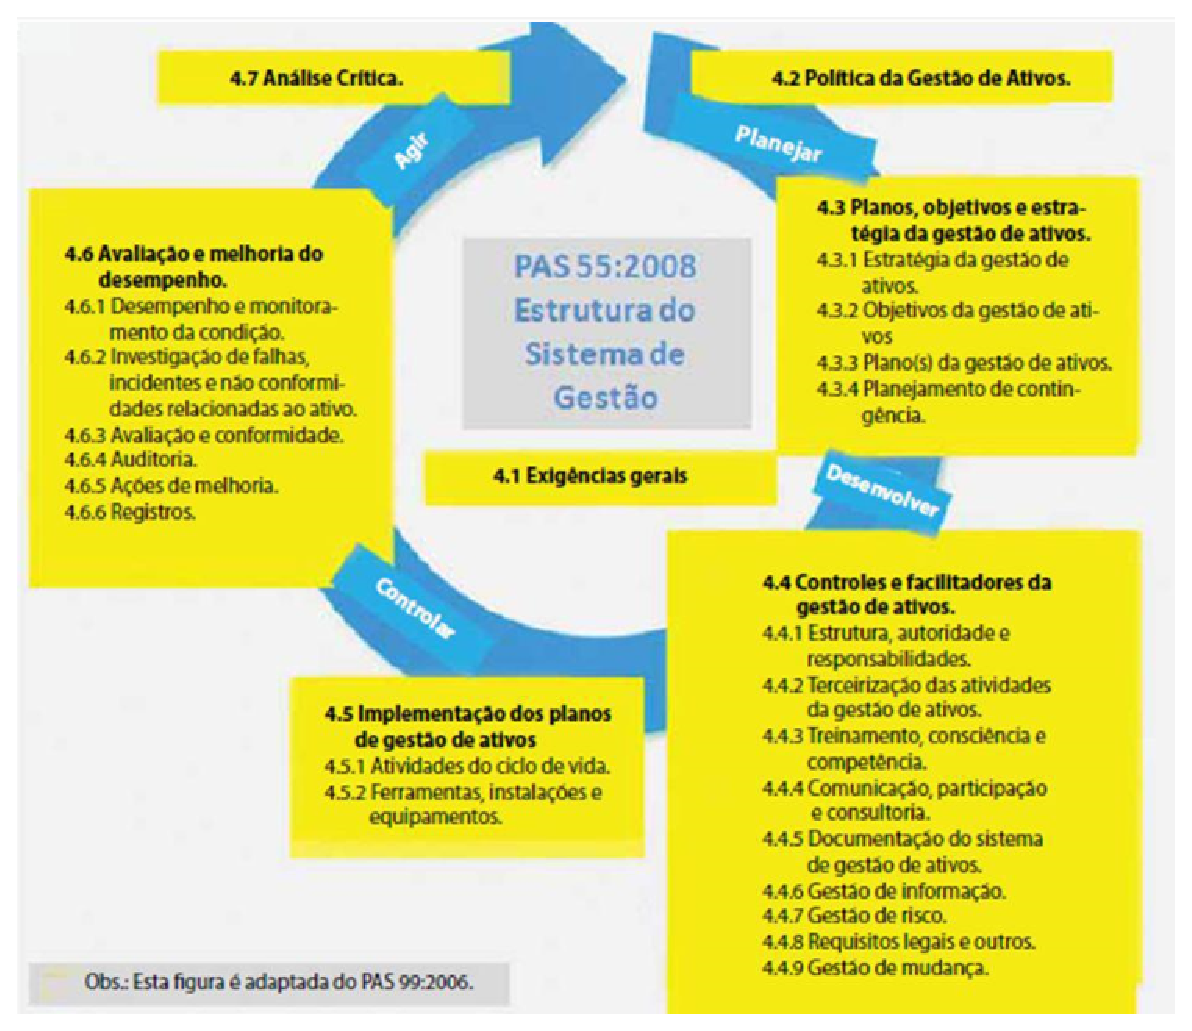
\includegraphics[width=1.0\textwidth]{pas55}
\caption{Estrutura do Sistema de Gestão de Ativos PAS 55. \textbf{Adaptado de: BSI PAS 55-1:2008.}}
\label{estrutura_pas_55}
\end{figure}

A Figura~\ref{estrutura_pas_55} foi adaptada por \cite{valeria2013} e mostra a estrutura do Sistema de Gestão de Ativos. A PAS classifica 5 categorias de ativos:

\begin{enumerate}
	\item{Ativos Físicos}
	\item{Ativos Humanos}
	\item{Ativos de Informação}
	\item{Ativos Financeiros}
	\item{Ativos Intangíveis}
\end{enumerate}

Contudo seu escopo está focado nos \textbf{ativos físicos}. Os outros só são considerados caso estejam relacionados a eles.

Segurança, confiabilidade, disponibilidade, infraestrutura e custo são associados a atividades contidas na gestão de ativos. 

Realizar a GA é importante para, conhecer a confiabilidade e a disponibilidade dos sistemas e componentes críticos ao longo do tempo de operação, os riscos inerentes à operação e manutenção, as probabilidades de ocorrências de eventos não desejáveis que afetem a segurança das pessoas e do meio-ambiente.


\subsection{ISO-5500x}

A importância da PAS 55 foi reconhecida quando baseada nela, em janeiro de 2014, foi aprovada a ISO-5500x, o primeiro padrão internacional para GA. 

A ISO é uma organização internacional e não governamental independente, tendo adesão de 161 organismos nacionais de normalização, sendo um deles a ABNT. Seu objetivo é construir padrões internacionais relevantes para o mercado e que deêm suporte a inovação e traga soluções para desafios globais.

O conjunto de normas ISO-5500x começou a ser elaborado em 2010 sendo aprovada em 2014. Foram aprovadas então três normas \cite{abraman}:

\begin{enumerate}
	\item \textbf{ISO-55000} (Visão geral, princípios e terminologia): Nela está contida a definição de Ativos, GA e SGA, e também os termos utilizados na área. Ela descreve quatro princípios para GA, sendo eles:
		\begin{enumerate}
			\item Ativos fornecem valores para a organização e interessados.
			\item GA transforma a estratégia definida pela organização em tarefas, decisões, atividades técnicas e financeiras.
			\item Liderança e cultura do local de trabalho são determinantes da percepção de valor.
			\item GA garante que os ativos vão cumprir e desempenhar a sua função.
		\end{enumerate}
	\item \textbf{ISO-55001} (Sistemas de Gestão - Requisitos): aborda quais os requisitos necessários para um SGA ser aplicado efetivamente. Ter uma maturidade no processo de GA não faz parte do seu escopo. É estabelecido aqui que a organização inclua como o valor pode ser proporcionado pelo SGA, e não se limita ao desempenho financeiro, à gestão de risco, ao desempenho de produção e de serviços. Cabe a organização escolher os fatores relevantes, assim como a escolha dos indicadores proativos e reativos
		\begin{enumerate}
			\item Fornece princípios, requisitos e orientações para um SGA.
			\item Aborda requisitos como a implantação dos princípios de GA e a documentação de quais ativos fazem parte do SGA e são escopo do Sistema de Gestão.
			\item Integra os processos decisórios com relação aos técnicos e financeiros.
			\item Destaca a implantação de um processo decisório com foco no balanceamento entre os fatores riscos, custos e desempenho dos ativos.
		\end{enumerate}
	\item \textbf{ISO-55002} (Sistemas de Gestão - Orientações para a aplicação da ISO 55001): provê um guia para a aplicação do SGA. 
\end{enumerate}

Na Figura~\ref{termos_iso_55000} são mostrados como os principais termos encontrados na norma 55000 se relacionam.

\graphicspath{{figuras/}}
\begin{figure}[H]
\centering
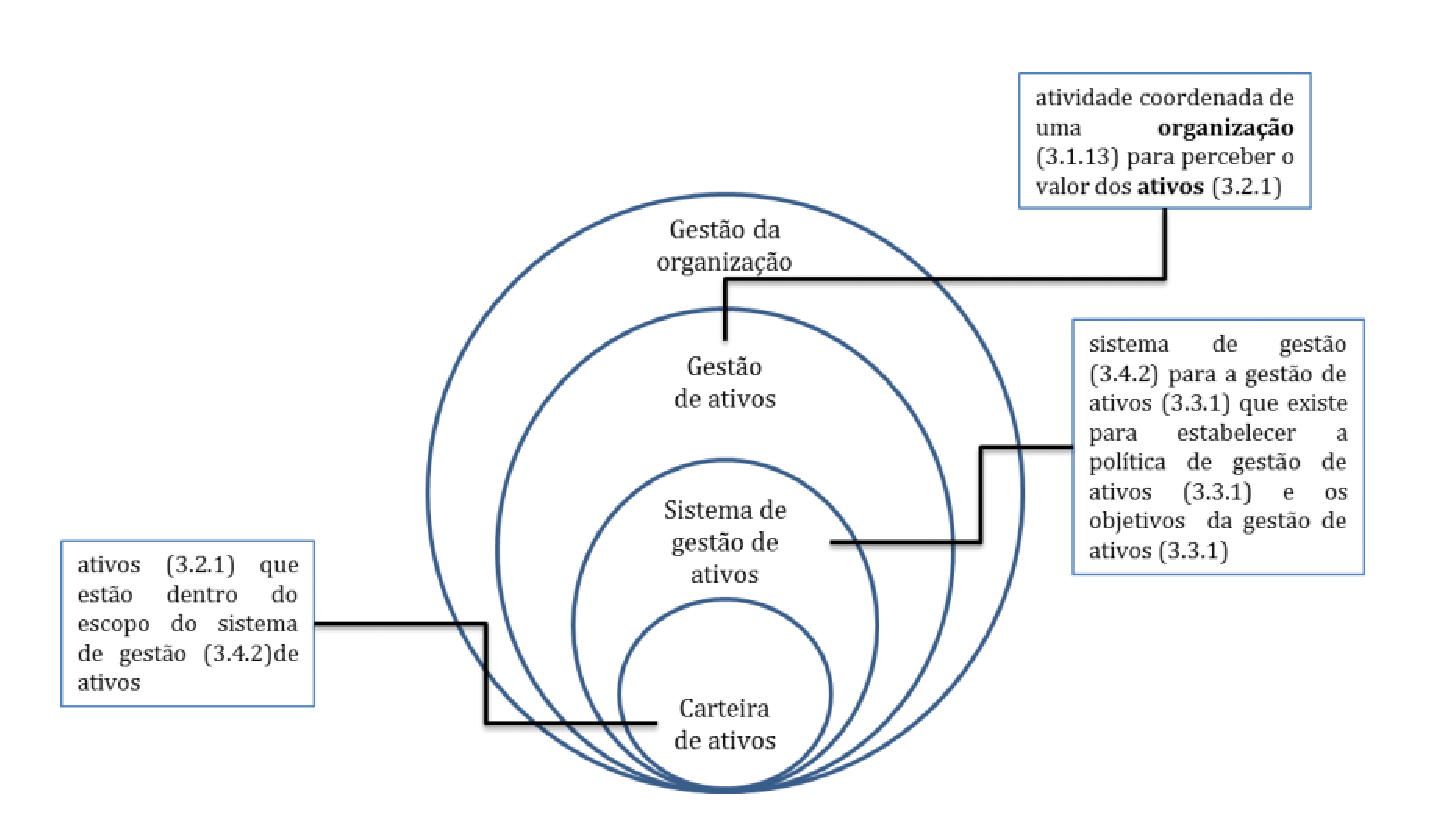
\includegraphics[width=1.0\textwidth]{termos_iso_55000.eps}
\caption{RELAÇÕES ENTRE OS PRINCIPAIS TERMOS da IS0-55000 \textbf{Fonte: Comissão de Estudo Especial de
Gestão de Ativos (ABNT/CEE-251).}}
\label{termos_iso_55000}
\end{figure}

Um dos pontos de melhoria da ISO em relação a PAS 55 Seção~\ref{pas55} é que ela fornece uma visão geral, explicando os princípios do GA, os quais podem trazer benefícios e oportunidade de alavancagem, por meio da integração com o gerenciamento de riscos e a governança da organização. 

João Ricardo Lafraia, CMRP, Presidente da ABRAMAN diz que \lq\lq \emph{o controle eficaz e governança de ativos por organizações é essencial para realizar o valor através de gerenciamento de riscos e oportunidades, a fim de alcançar o equilíbrio desejado de custo, risco e desempenho}\rq\rq, mostrando a importância de se ter uma GA integrada com as outras partes da organização para que assim seja possível ver que uma GA efetiva e eficiente pode gerar valor de negócio na organização não só financeiro, mas também para uma melhor estruturação e realização de suas atividades. 


